\documentclass[../main.tex]{subfiles}

\begin{document}
\begin{enumerate}[a)]
    \item Para dibujar el perfil de temperatura consideramos que la capa limite tiene un ancho de 100 hPa ( desde los 1000 hasta los 900 hPa), y que al estar mezclada mantiene constante su temperatura potencial. Nos dicen que en la superficie (la que consideramos en los 1000 hPa) presenta una temperatura de 15$^{\circ}$C, por lo que a partir de ese punto el perfil sube siguiendo la curva adiabática seca. 

        Al llegar a los 900 hPa tenemos una discontinuidad o salto en 10$^{\circ}$C y luego seguimos ascendiendo pero ahora con un gradiente de temperatura de -5 $^{\circ}$C por cada 100 hPa, hasta llegar a los 500 hPa.

        Para estimar el perfil de la temperatura punto de rocío, consideramos que en la superficie la humedad relativa es del 50$\%$. Con este dato ( y considerando que el perfil de temperatura en la superficie indican una razon de mezcla saturada de  $w_\text{sat}\simeq 10.5$ g/Kg) obtenemos que la razón de mezcla de la parcela es $w \simeq 5.25$ g/Kg en la superficie. Luego, como la capa límite está mezclada también asumimos que la razón de mezcla se mantiene constante, de modo que el perfil de la temperatura punto de rocío sube con razón de mezcla constante hasta los 900 hPa.

Nos mencionan que en la troposfera libre la razón de mezcla es constante en 1 g/Kg, por lo que el la temperatura punto de rocío sigue esa linea de razón de mezcla constante.\\

\begin{minipage}{\linewidth}
    \begin{center}
        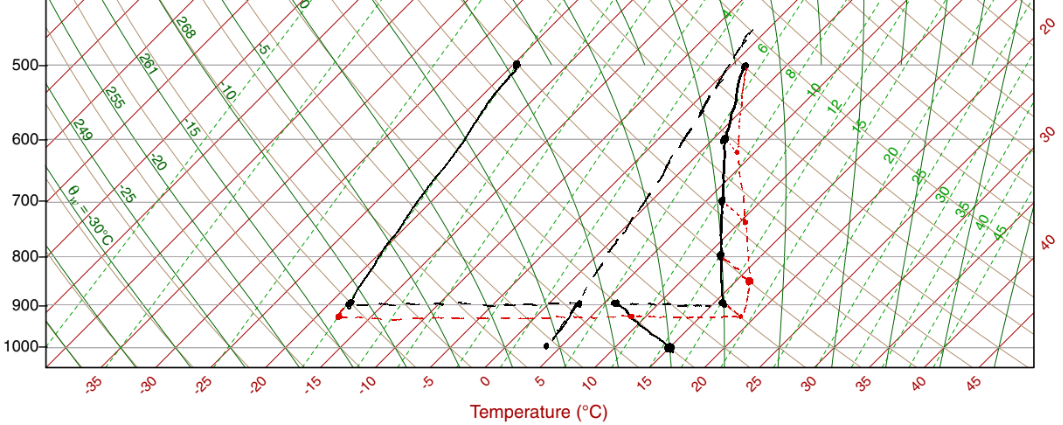
\includegraphics[width=0.8\textwidth]{img/skewT}
        \captionof{figure}{Perfiles de temperatura. La linea continua negra de la derecha representa el perfil de temperatura, mientras que la de la izquierda corresponde a la temperatura punto de rocío. Las lineas rojas corresponden a las temperaturas luego de que se aplica el descenso. }
        \label{skewT}
    \end{center}
\end{minipage}\\

Para dibujar el descenso, se consideraron varios puntos en el perfil de temperatura (puntos negros), que se hicieron descender por trayectorias adiabáticas secas. El descenso (en hPa) para cada punto fue estimado acorde al perfil de descenso del enunciado, en donde el punto a 800 hPa, presenta el mayor descenso (de unos 50 hPa). Con este procedimiento se obtuvieron los punto rojos de la figura \eqref{skewT}, y luego unimos ( interpolamos? ) los puntos rojos para hacernos una idea de como queda el perfil luego del descenso.
\end{enumerate}


\end{document}
